% J. R. Capablanca - R. Teichmann, Berlin, 1913, with Capablanca's notes.
% Build with: python3 ../../tools/chessbook.py game-09-capablanca-teichmann.tex
\documentclass[10pt,twoside]{article}
\usepackage[paperwidth=487.56bp,paperheight=691.65bp,top=72pt,bottom=44pt,inner=50pt,outer=48pt,
            headheight=13pt,headsep=20pt,footskip=0pt]{geometry}
\usepackage[T1]{fontenc}
\usepackage[lining]{ebgaramond}
\usepackage{graphicx}
\usepackage{microtype}
\usepackage{tikz}
\usepackage{fancyhdr}
\usepackage[hidelinks,pdftitle={Capablanca - Teichmann, Berlin, 1913},
            pdfauthor={J. R. Capablanca}]{hyperref}

\newcommand{\textsizebook}{\fontsize{10.5}{12.6}\selectfont}
\AtBeginDocument{\textsizebook}
\setlength{\columnsep}{11pt}
\setlength{\parindent}{9pt}
\setlength{\parskip}{0pt}
\setlength{\emergencystretch}{1.5em}
\raggedbottom

\newlength{\boardwidth}
\setlength{\boardwidth}{160pt}

% A main line move, as a bold heading above its note
\newcommand{\Move}[1]{\par\addvspace{8pt}\noindent\phantomsection{\bfseries #1}\par\nopagebreak}
% A diagram in the text
\newcommand{\ChessDiagram}[1]{\par\addvspace{7pt}{\centering #1\par}\addvspace{5pt}}

\pagestyle{fancy}
\fancyhf{}
\renewcommand{\headrulewidth}{0pt}
\fancyhead[LE,RO]{\thepage}
\fancyhead[CE]{Queen's Gambit Declined}
\fancyhead[CO]{Capablanca -- Teichmann}






\newcommand{\figK}{\raisebox{-0.14em}{
\includegraphics[height=1em]{diagrams/figK}}}
\newcommand{\figQ}{\raisebox{-0.14em}{
\includegraphics[height=1em]{diagrams/figQ}}}
\newcommand{\figR}{\raisebox{-0.14em}{
\includegraphics[height=1em]{diagrams/figR}}}
\newcommand{\figB}{\raisebox{-0.14em}{
\includegraphics[height=1em]{diagrams/figB}}}
\newcommand{\figN}{\raisebox{-0.14em}{
\includegraphics[height=1em]{diagrams/figN}}}
\begin{document}

\twocolumn[{%
\thispagestyle{empty}
\begin{tikzpicture}[remember picture,overlay]
  \node[circle,draw=black,line width=1.6pt,fill=black!20,minimum size=112pt] (seal)
       at ([xshift=75pt,yshift=-75pt]current page.north west) {};
  \draw[line width=0.9pt] ([shift={(-48pt,-30pt)}]seal.center) -- ([shift={(44pt,34pt)}]seal.center);
  \node[rotate=37] at ([shift={(-11pt,14pt)}]seal.center) {\fontsize{25}{25}\selectfont\bfseries Game};
  \node[rotate=37] at ([shift={(10pt,-16pt)}]seal.center) {\fontsize{38}{38}\selectfont\bfseries 9};
  \node[anchor=north east] at ([xshift=-14pt,yshift=-24pt]current page.north east)
       {\href{https://lichess.org/analysis/pgn/d4_d5_Nf3_Nf6_c4_e6_Bg5_Be7}{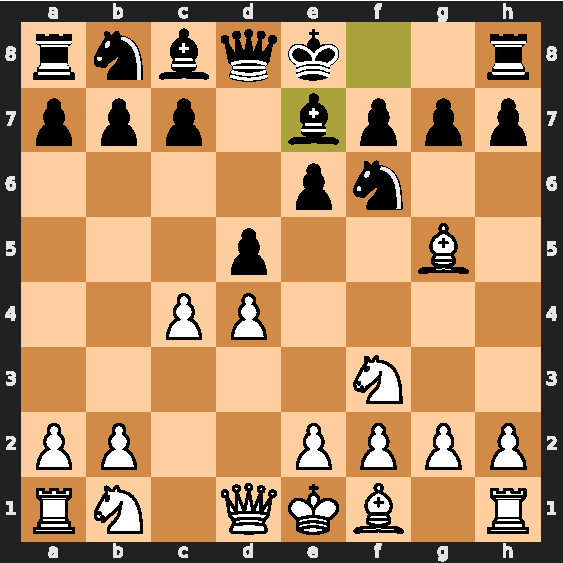
\includegraphics[width=108pt]{diagrams/board-538c4211d134}}};
\end{tikzpicture}

\vspace*{38pt}
\begin{center}
  \begin{minipage}{235pt}\centering
    {\fontsize{22}{25}\selectfont\bfseries Queen's Gambit Declined\par}
    \vspace{4pt}\rule{\linewidth}{1pt}\\[-9.5pt]\rule{\linewidth}{0.4pt}
  \end{minipage}

  \vspace{14pt}
  {\fontsize{19}{22}\selectfont\bfseries Capablanca -- Teichmann\par}
  \vspace{10pt}
  {\fontsize{15}{18}\selectfont\bfseries Berlin, 1913\par}
  \vspace{8pt}
  {\fontsize{11}{13}\selectfont White: J. R. Capablanca \quad Black: R. Teichmann\par}
  \vspace{10pt}
  {\centering\fontsize{8.5}{10}\selectfont\itshape
   Notes by J. R. Capablanca, from \textup{Chess Fundamentals} (1921), which is in the public domain.\\
   Descriptive notation has been converted to algebraic. Page references are to the book.\\
   Click any move or diagram to open it on Lichess.\par}
\end{center}
\vspace{10pt}
}]
\textsizebook

\Move{\href{https://lichess.org/analysis/pgn/d4}{1.d4} \href{https://lichess.org/analysis/pgn/d4_d5}{d5} \href{https://lichess.org/analysis/pgn/d4_d5_Nf3}{2.\figN f3} \href{https://lichess.org/analysis/pgn/d4_d5_Nf3_Nf6}{\figN f6} \href{https://lichess.org/analysis/pgn/d4_d5_Nf3_Nf6_c4}{3.c4} \href{https://lichess.org/analysis/pgn/d4_d5_Nf3_Nf6_c4_e6}{e6} \href{https://lichess.org/analysis/pgn/d4_d5_Nf3_Nf6_c4_e6_Bg5}{4.\figB g5} \href{https://lichess.org/analysis/pgn/d4_d5_Nf3_Nf6_c4_e6_Bg5_Be7}{\figB e7} \href{https://lichess.org/analysis/pgn/d4_d5_Nf3_Nf6_c4_e6_Bg5_Be7_Nc3}{5.\figN c3} \href{https://lichess.org/analysis/pgn/d4_d5_Nf3_Nf6_c4_e6_Bg5_Be7_Nc3_Nbd7}{\figN bd7} \href{https://lichess.org/analysis/pgn/d4_d5_Nf3_Nf6_c4_e6_Bg5_Be7_Nc3_Nbd7_e3}{6.e3} \href{https://lichess.org/analysis/pgn/d4_d5_Nf3_Nf6_c4_e6_Bg5_Be7_Nc3_Nbd7_e3_O-O}{0--0} \href{https://lichess.org/analysis/pgn/d4_d5_Nf3_Nf6_c4_e6_Bg5_Be7_Nc3_Nbd7_e3_O-O_Rc1}{7.\figR c1} \href{https://lichess.org/analysis/pgn/d4_d5_Nf3_Nf6_c4_e6_Bg5_Be7_Nc3_Nbd7_e3_O-O_Rc1_b6}{b6} \href{https://lichess.org/analysis/pgn/d4_d5_Nf3_Nf6_c4_e6_Bg5_Be7_Nc3_Nbd7_e3_O-O_Rc1_b6_cxd5}{8.cxd5} \href{https://lichess.org/analysis/pgn/d4_d5_Nf3_Nf6_c4_e6_Bg5_Be7_Nc3_Nbd7_e3_O-O_Rc1_b6_cxd5_exd5}{exd5} \href{https://lichess.org/analysis/pgn/d4_d5_Nf3_Nf6_c4_e6_Bg5_Be7_Nc3_Nbd7_e3_O-O_Rc1_b6_cxd5_exd5_Bb5}{9.\figB b5}}

An invention of my own, I believe. I played it on the spur of the moment simply to change the normal course of the game. Generally the Bishop goes to d3, or to a6, after \href{https://lichess.org/analysis/pgn/d4_d5_Nf3_Nf6_c4_e6_Bg5_Be7_Nc3_Nbd7_e3_O-O_Rc1_b6_cxd5_exd5_Qa4}{9.\figQ a4}. The text move is in the nature of an ordinary developing move, and as it violates no principle it cannot be bad.

\Move{\href{https://lichess.org/analysis/pgn/d4_d5_Nf3_Nf6_c4_e6_Bg5_Be7_Nc3_Nbd7_e3_O-O_Rc1_b6_cxd5_exd5_Bb5_Bb7}{9...\figB b7} \href{https://lichess.org/analysis/pgn/d4_d5_Nf3_Nf6_c4_e6_Bg5_Be7_Nc3_Nbd7_e3_O-O_Rc1_b6_cxd5_exd5_Bb5_Bb7_O-O}{10.0--0} \href{https://lichess.org/analysis/pgn/d4_d5_Nf3_Nf6_c4_e6_Bg5_Be7_Nc3_Nbd7_e3_O-O_Rc1_b6_cxd5_exd5_Bb5_Bb7_O-O_a6}{a6} \href{https://lichess.org/analysis/pgn/d4_d5_Nf3_Nf6_c4_e6_Bg5_Be7_Nc3_Nbd7_e3_O-O_Rc1_b6_cxd5_exd5_Bb5_Bb7_O-O_a6_Ba4}{11.\figB a4} \href{https://lichess.org/analysis/pgn/d4_d5_Nf3_Nf6_c4_e6_Bg5_Be7_Nc3_Nbd7_e3_O-O_Rc1_b6_cxd5_exd5_Bb5_Bb7_O-O_a6_Ba4_Rc8}{\figR c8} \href{https://lichess.org/analysis/pgn/d4_d5_Nf3_Nf6_c4_e6_Bg5_Be7_Nc3_Nbd7_e3_O-O_Rc1_b6_cxd5_exd5_Bb5_Bb7_O-O_a6_Ba4_Rc8_Qe2}{12.\figQ e2} \href{https://lichess.org/analysis/pgn/d4_d5_Nf3_Nf6_c4_e6_Bg5_Be7_Nc3_Nbd7_e3_O-O_Rc1_b6_cxd5_exd5_Bb5_Bb7_O-O_a6_Ba4_Rc8_Qe2_c5}{c5} \href{https://lichess.org/analysis/pgn/d4_d5_Nf3_Nf6_c4_e6_Bg5_Be7_Nc3_Nbd7_e3_O-O_Rc1_b6_cxd5_exd5_Bb5_Bb7_O-O_a6_Ba4_Rc8_Qe2_c5_dxc5}{13.dxc5} \href{https://lichess.org/analysis/pgn/d4_d5_Nf3_Nf6_c4_e6_Bg5_Be7_Nc3_Nbd7_e3_O-O_Rc1_b6_cxd5_exd5_Bb5_Bb7_O-O_a6_Ba4_Rc8_Qe2_c5_dxc5_Nxc5}{\figN xc5}}

If \href{https://lichess.org/analysis/pgn/d4_d5_Nf3_Nf6_c4_e6_Bg5_Be7_Nc3_Nbd7_e3_O-O_Rc1_b6_cxd5_exd5_Bb5_Bb7_O-O_a6_Ba4_Rc8_Qe2_c5_dxc5_bxc5}{13...bxc5} \href{https://lichess.org/analysis/pgn/d4_d5_Nf3_Nf6_c4_e6_Bg5_Be7_Nc3_Nbd7_e3_O-O_Rc1_b6_cxd5_exd5_Bb5_Bb7_O-O_a6_Ba4_Rc8_Qe2_c5_dxc5_bxc5_Rfd1}{14.\figR fd1}, and White would play to win one of Black's centre Pawns. The drawback to the text move is that it leaves Black's d-pawn isolated, and consequently weak and subject to attack.

\Move{\href{https://lichess.org/analysis/pgn/d4_d5_Nf3_Nf6_c4_e6_Bg5_Be7_Nc3_Nbd7_e3_O-O_Rc1_b6_cxd5_exd5_Bb5_Bb7_O-O_a6_Ba4_Rc8_Qe2_c5_dxc5_Nxc5_Rfd1}{14.\figR fd1} \href{https://lichess.org/analysis/pgn/d4_d5_Nf3_Nf6_c4_e6_Bg5_Be7_Nc3_Nbd7_e3_O-O_Rc1_b6_cxd5_exd5_Bb5_Bb7_O-O_a6_Ba4_Rc8_Qe2_c5_dxc5_Nxc5_Rfd1_Nxa4}{\figN xa4}}

The alternative would have been \href{https://lichess.org/analysis/pgn/d4_d5_Nf3_Nf6_c4_e6_Bg5_Be7_Nc3_Nbd7_e3_O-O_Rc1_b6_cxd5_exd5_Bb5_Bb7_O-O_a6_Ba4_Rc8_Qe2_c5_dxc5_Nxc5_Rfd1_b5}{14...b5} \href{https://lichess.org/analysis/pgn/d4_d5_Nf3_Nf6_c4_e6_Bg5_Be7_Nc3_Nbd7_e3_O-O_Rc1_b6_cxd5_exd5_Bb5_Bb7_O-O_a6_Ba4_Rc8_Qe2_c5_dxc5_Nxc5_Rfd1_b5_Bc2}{15.\figB c2} \href{https://lichess.org/analysis/pgn/d4_d5_Nf3_Nf6_c4_e6_Bg5_Be7_Nc3_Nbd7_e3_O-O_Rc1_b6_cxd5_exd5_Bb5_Bb7_O-O_a6_Ba4_Rc8_Qe2_c5_dxc5_Nxc5_Rfd1_b5_Bc2_b4}{b4} \href{https://lichess.org/analysis/pgn/d4_d5_Nf3_Nf6_c4_e6_Bg5_Be7_Nc3_Nbd7_e3_O-O_Rc1_b6_cxd5_exd5_Bb5_Bb7_O-O_a6_Ba4_Rc8_Qe2_c5_dxc5_Nxc5_Rfd1_b5_Bc2_b4_Na4}{16.\figN a4} \href{https://lichess.org/analysis/pgn/d4_d5_Nf3_Nf6_c4_e6_Bg5_Be7_Nc3_Nbd7_e3_O-O_Rc1_b6_cxd5_exd5_Bb5_Bb7_O-O_a6_Ba4_Rc8_Qe2_c5_dxc5_Nxc5_Rfd1_b5_Bc2_b4_Na4_Nce4}{\figN ce4}.

\Move{\href{https://lichess.org/analysis/pgn/d4_d5_Nf3_Nf6_c4_e6_Bg5_Be7_Nc3_Nbd7_e3_O-O_Rc1_b6_cxd5_exd5_Bb5_Bb7_O-O_a6_Ba4_Rc8_Qe2_c5_dxc5_Nxc5_Rfd1_Nxa4_Nxa4}{15.\figN xa4} \href{https://lichess.org/analysis/pgn/d4_d5_Nf3_Nf6_c4_e6_Bg5_Be7_Nc3_Nbd7_e3_O-O_Rc1_b6_cxd5_exd5_Bb5_Bb7_O-O_a6_Ba4_Rc8_Qe2_c5_dxc5_Nxc5_Rfd1_Nxa4_Nxa4_b5}{b5} \href{https://lichess.org/analysis/pgn/d4_d5_Nf3_Nf6_c4_e6_Bg5_Be7_Nc3_Nbd7_e3_O-O_Rc1_b6_cxd5_exd5_Bb5_Bb7_O-O_a6_Ba4_Rc8_Qe2_c5_dxc5_Nxc5_Rfd1_Nxa4_Nxa4_b5_Rxc8}{16.\figR xc8} \href{https://lichess.org/analysis/pgn/d4_d5_Nf3_Nf6_c4_e6_Bg5_Be7_Nc3_Nbd7_e3_O-O_Rc1_b6_cxd5_exd5_Bb5_Bb7_O-O_a6_Ba4_Rc8_Qe2_c5_dxc5_Nxc5_Rfd1_Nxa4_Nxa4_b5_Rxc8_Qxc8}{\figQ xc8} \href{https://lichess.org/analysis/pgn/d4_d5_Nf3_Nf6_c4_e6_Bg5_Be7_Nc3_Nbd7_e3_O-O_Rc1_b6_cxd5_exd5_Bb5_Bb7_O-O_a6_Ba4_Rc8_Qe2_c5_dxc5_Nxc5_Rfd1_Nxa4_Nxa4_b5_Rxc8_Qxc8_Nc3}{17.\figN c3} \href{https://lichess.org/analysis/pgn/d4_d5_Nf3_Nf6_c4_e6_Bg5_Be7_Nc3_Nbd7_e3_O-O_Rc1_b6_cxd5_exd5_Bb5_Bb7_O-O_a6_Ba4_Rc8_Qe2_c5_dxc5_Nxc5_Rfd1_Nxa4_Nxa4_b5_Rxc8_Qxc8_Nc3_Qc4}{\figQ c4}}

Black aims at the exchange of Queens in order to remain with two Bishops for the ending, but in this position such a course is a mistake, because the Bishop at b7 is inactive and cannot come into the game by any means, unless Black gives up the isolated Queen's Pawn which the Bishop must defend.

\Move{\href{https://lichess.org/analysis/pgn/d4_d5_Nf3_Nf6_c4_e6_Bg5_Be7_Nc3_Nbd7_e3_O-O_Rc1_b6_cxd5_exd5_Bb5_Bb7_O-O_a6_Ba4_Rc8_Qe2_c5_dxc5_Nxc5_Rfd1_Nxa4_Nxa4_b5_Rxc8_Qxc8_Nc3_Qc4_Nd4}{18.\figN d4}}

Not, of course, \href{https://lichess.org/analysis/pgn/d4_d5_Nf3_Nf6_c4_e6_Bg5_Be7_Nc3_Nbd7_e3_O-O_Rc1_b6_cxd5_exd5_Bb5_Bb7_O-O_a6_Ba4_Rc8_Qe2_c5_dxc5_Nxc5_Rfd1_Nxa4_Nxa4_b5_Rxc8_Qxc8_Nc3_Qc4_Rd4}{18.\figR d4}, because of \href{https://lichess.org/analysis/pgn/d4_d5_Nf3_Nf6_c4_e6_Bg5_Be7_Nc3_Nbd7_e3_O-O_Rc1_b6_cxd5_exd5_Bb5_Bb7_O-O_a6_Ba4_Rc8_Qe2_c5_dxc5_Nxc5_Rfd1_Nxa4_Nxa4_b5_Rxc8_Qxc8_Nc3_Qc4_Rd4_Qxe2}{18...\figQ xe2} \href{https://lichess.org/analysis/pgn/d4_d5_Nf3_Nf6_c4_e6_Bg5_Be7_Nc3_Nbd7_e3_O-O_Rc1_b6_cxd5_exd5_Bb5_Bb7_O-O_a6_Ba4_Rc8_Qe2_c5_dxc5_Nxc5_Rfd1_Nxa4_Nxa4_b5_Rxc8_Qxc8_Nc3_Qc4_Rd4_Qxe2_Nxe2}{19.\figN xe2} \href{https://lichess.org/analysis/pgn/d4_d5_Nf3_Nf6_c4_e6_Bg5_Be7_Nc3_Nbd7_e3_O-O_Rc1_b6_cxd5_exd5_Bb5_Bb7_O-O_a6_Ba4_Rc8_Qe2_c5_dxc5_Nxc5_Rfd1_Nxa4_Nxa4_b5_Rxc8_Qxc8_Nc3_Qc4_Rd4_Qxe2_Nxe2_Rc8}{\figR c8}; and there would be no good way to prevent \figR c2.

\Move{\href{https://lichess.org/analysis/pgn/d4_d5_Nf3_Nf6_c4_e6_Bg5_Be7_Nc3_Nbd7_e3_O-O_Rc1_b6_cxd5_exd5_Bb5_Bb7_O-O_a6_Ba4_Rc8_Qe2_c5_dxc5_Nxc5_Rfd1_Nxa4_Nxa4_b5_Rxc8_Qxc8_Nc3_Qc4_Nd4_Qxe2}{18...\figQ xe2} \href{https://lichess.org/analysis/pgn/d4_d5_Nf3_Nf6_c4_e6_Bg5_Be7_Nc3_Nbd7_e3_O-O_Rc1_b6_cxd5_exd5_Bb5_Bb7_O-O_a6_Ba4_Rc8_Qe2_c5_dxc5_Nxc5_Rfd1_Nxa4_Nxa4_b5_Rxc8_Qxc8_Nc3_Qc4_Nd4_Qxe2_Ncxe2}{19.\figN cxe2!}}

Notice the co-ordination of the Knights' moves. They are manoeuvred chain-like, so to speak, in order to maintain one of them, either at d4 or ready to go there. Now White threatens to take the open file, and therefore forces Black's next move.

\Move{\href{https://lichess.org/analysis/pgn/d4_d5_Nf3_Nf6_c4_e6_Bg5_Be7_Nc3_Nbd7_e3_O-O_Rc1_b6_cxd5_exd5_Bb5_Bb7_O-O_a6_Ba4_Rc8_Qe2_c5_dxc5_Nxc5_Rfd1_Nxa4_Nxa4_b5_Rxc8_Qxc8_Nc3_Qc4_Nd4_Qxe2_Ncxe2_Rc8}{19...\figR c8}}

\ChessDiagram{\href{https://lichess.org/analysis/pgn/d4_d5_Nf3_Nf6_c4_e6_Bg5_Be7_Nc3_Nbd7_e3_O-O_Rc1_b6_cxd5_exd5_Bb5_Bb7_O-O_a6_Ba4_Rc8_Qe2_c5_dxc5_Nxc5_Rfd1_Nxa4_Nxa4_b5_Rxc8_Qxc8_Nc3_Qc4_Nd4_Qxe2_Ncxe2_Rc8}{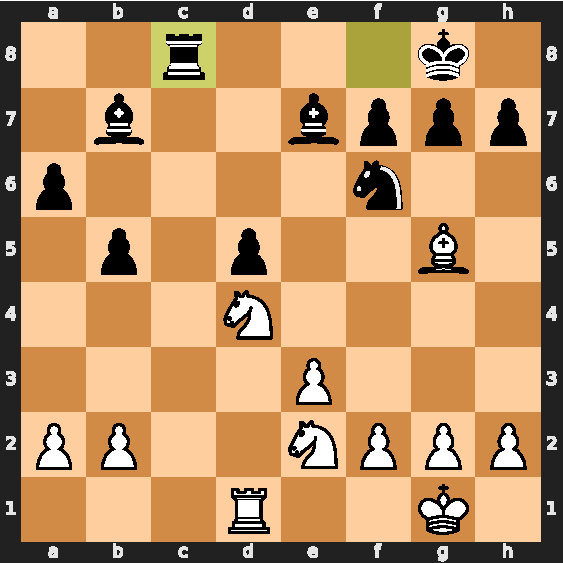
\includegraphics[width=\boardwidth]{diagrams/board-bbcf9757c83a}}}

The student should examine this position carefully. There seems to be no particular danger, yet, as White will demonstrate, Black may be said to be lost. If the game is not altogether lost, the defence is at least of the most difficult kind; indeed, I must confess that I can see no adequate defence against White's next move.

\Move{\href{https://lichess.org/analysis/pgn/d4_d5_Nf3_Nf6_c4_e6_Bg5_Be7_Nc3_Nbd7_e3_O-O_Rc1_b6_cxd5_exd5_Bb5_Bb7_O-O_a6_Ba4_Rc8_Qe2_c5_dxc5_Nxc5_Rfd1_Nxa4_Nxa4_b5_Rxc8_Qxc8_Nc3_Qc4_Nd4_Qxe2_Ncxe2_Rc8_Nf5}{20.\figN f5!} \href{https://lichess.org/analysis/pgn/d4_d5_Nf3_Nf6_c4_e6_Bg5_Be7_Nc3_Nbd7_e3_O-O_Rc1_b6_cxd5_exd5_Bb5_Bb7_O-O_a6_Ba4_Rc8_Qe2_c5_dxc5_Nxc5_Rfd1_Nxa4_Nxa4_b5_Rxc8_Qxc8_Nc3_Qc4_Nd4_Qxe2_Ncxe2_Rc8_Nf5_Kf8}{\figK f8}}

If \href{https://lichess.org/analysis/pgn/d4_d5_Nf3_Nf6_c4_e6_Bg5_Be7_Nc3_Nbd7_e3_O-O_Rc1_b6_cxd5_exd5_Bb5_Bb7_O-O_a6_Ba4_Rc8_Qe2_c5_dxc5_Nxc5_Rfd1_Nxa4_Nxa4_b5_Rxc8_Qxc8_Nc3_Qc4_Nd4_Qxe2_Ncxe2_Rc8_Nf5_Bd8}{20...\figB d8} \href{https://lichess.org/analysis/pgn/d4_d5_Nf3_Nf6_c4_e6_Bg5_Be7_Nc3_Nbd7_e3_O-O_Rc1_b6_cxd5_exd5_Bb5_Bb7_O-O_a6_Ba4_Rc8_Qe2_c5_dxc5_Nxc5_Rfd1_Nxa4_Nxa4_b5_Rxc8_Qxc8_Nc3_Qc4_Nd4_Qxe2_Ncxe2_Rc8_Nf5_Bd8_Nd6}{21.\figN d6} \href{https://lichess.org/analysis/pgn/d4_d5_Nf3_Nf6_c4_e6_Bg5_Be7_Nc3_Nbd7_e3_O-O_Rc1_b6_cxd5_exd5_Bb5_Bb7_O-O_a6_Ba4_Rc8_Qe2_c5_dxc5_Nxc5_Rfd1_Nxa4_Nxa4_b5_Rxc8_Qxc8_Nc3_Qc4_Nd4_Qxe2_Ncxe2_Rc8_Nf5_Bd8_Nd6_Rc7}{\figR c7} \href{https://lichess.org/analysis/pgn/d4_d5_Nf3_Nf6_c4_e6_Bg5_Be7_Nc3_Nbd7_e3_O-O_Rc1_b6_cxd5_exd5_Bb5_Bb7_O-O_a6_Ba4_Rc8_Qe2_c5_dxc5_Nxc5_Rfd1_Nxa4_Nxa4_b5_Rxc8_Qxc8_Nc3_Qc4_Nd4_Qxe2_Ncxe2_Rc8_Nf5_Bd8_Nd6_Rc7_Nxb7}{22.\figN xb7} \href{https://lichess.org/analysis/pgn/d4_d5_Nf3_Nf6_c4_e6_Bg5_Be7_Nc3_Nbd7_e3_O-O_Rc1_b6_cxd5_exd5_Bb5_Bb7_O-O_a6_Ba4_Rc8_Qe2_c5_dxc5_Nxc5_Rfd1_Nxa4_Nxa4_b5_Rxc8_Qxc8_Nc3_Qc4_Nd4_Qxe2_Ncxe2_Rc8_Nf5_Bd8_Nd6_Rc7_Nxb7_Rxb7}{\figR xb7} \href{https://lichess.org/analysis/pgn/d4_d5_Nf3_Nf6_c4_e6_Bg5_Be7_Nc3_Nbd7_e3_O-O_Rc1_b6_cxd5_exd5_Bb5_Bb7_O-O_a6_Ba4_Rc8_Qe2_c5_dxc5_Nxc5_Rfd1_Nxa4_Nxa4_b5_Rxc8_Qxc8_Nc3_Qc4_Nd4_Qxe2_Ncxe2_Rc8_Nf5_Bd8_Nd6_Rc7_Nxb7_Rxb7_Bxf6}{23.\figB xf6} \href{https://lichess.org/analysis/pgn/d4_d5_Nf3_Nf6_c4_e6_Bg5_Be7_Nc3_Nbd7_e3_O-O_Rc1_b6_cxd5_exd5_Bb5_Bb7_O-O_a6_Ba4_Rc8_Qe2_c5_dxc5_Nxc5_Rfd1_Nxa4_Nxa4_b5_Rxc8_Qxc8_Nc3_Qc4_Nd4_Qxe2_Ncxe2_Rc8_Nf5_Bd8_Nd6_Rc7_Nxb7_Rxb7_Bxf6_Bxf6}{\figB xf6} \href{https://lichess.org/analysis/pgn/d4_d5_Nf3_Nf6_c4_e6_Bg5_Be7_Nc3_Nbd7_e3_O-O_Rc1_b6_cxd5_exd5_Bb5_Bb7_O-O_a6_Ba4_Rc8_Qe2_c5_dxc5_Nxc5_Rfd1_Nxa4_Nxa4_b5_Rxc8_Qxc8_Nc3_Qc4_Nd4_Qxe2_Ncxe2_Rc8_Nf5_Bd8_Nd6_Rc7_Nxb7_Rxb7_Bxf6_Bxf6_Rxd5}{24.\figR xd5} \href{https://lichess.org/analysis/pgn/d4_d5_Nf3_Nf6_c4_e6_Bg5_Be7_Nc3_Nbd7_e3_O-O_Rc1_b6_cxd5_exd5_Bb5_Bb7_O-O_a6_Ba4_Rc8_Qe2_c5_dxc5_Nxc5_Rfd1_Nxa4_Nxa4_b5_Rxc8_Qxc8_Nc3_Qc4_Nd4_Qxe2_Ncxe2_Rc8_Nf5_Bd8_Nd6_Rc7_Nxb7_Rxb7_Bxf6_Bxf6_Rxd5_Rc7}{\figR c7} \href{https://lichess.org/analysis/pgn/d4_d5_Nf3_Nf6_c4_e6_Bg5_Be7_Nc3_Nbd7_e3_O-O_Rc1_b6_cxd5_exd5_Bb5_Bb7_O-O_a6_Ba4_Rc8_Qe2_c5_dxc5_Nxc5_Rfd1_Nxa4_Nxa4_b5_Rxc8_Qxc8_Nc3_Qc4_Nd4_Qxe2_Ncxe2_Rc8_Nf5_Bd8_Nd6_Rc7_Nxb7_Rxb7_Bxf6_Bxf6_Rxd5_Rc7_Rd2}{25.\figR d2}, and White is a Pawn ahead. If the Bishop moves anywhere else, then \figB xf6, doubling the f-pawn and isolating all of Black's King's side Pawns.

\Move{\href{https://lichess.org/analysis/pgn/d4_d5_Nf3_Nf6_c4_e6_Bg5_Be7_Nc3_Nbd7_e3_O-O_Rc1_b6_cxd5_exd5_Bb5_Bb7_O-O_a6_Ba4_Rc8_Qe2_c5_dxc5_Nxc5_Rfd1_Nxa4_Nxa4_b5_Rxc8_Qxc8_Nc3_Qc4_Nd4_Qxe2_Ncxe2_Rc8_Nf5_Kf8_Nxe7}{21.\figN xe7} \href{https://lichess.org/analysis/pgn/d4_d5_Nf3_Nf6_c4_e6_Bg5_Be7_Nc3_Nbd7_e3_O-O_Rc1_b6_cxd5_exd5_Bb5_Bb7_O-O_a6_Ba4_Rc8_Qe2_c5_dxc5_Nxc5_Rfd1_Nxa4_Nxa4_b5_Rxc8_Qxc8_Nc3_Qc4_Nd4_Qxe2_Ncxe2_Rc8_Nf5_Kf8_Nxe7_Kxe7}{\figK xe7} \href{https://lichess.org/analysis/pgn/d4_d5_Nf3_Nf6_c4_e6_Bg5_Be7_Nc3_Nbd7_e3_O-O_Rc1_b6_cxd5_exd5_Bb5_Bb7_O-O_a6_Ba4_Rc8_Qe2_c5_dxc5_Nxc5_Rfd1_Nxa4_Nxa4_b5_Rxc8_Qxc8_Nc3_Qc4_Nd4_Qxe2_Ncxe2_Rc8_Nf5_Kf8_Nxe7_Kxe7_Nd4}{22.\figN d4} \href{https://lichess.org/analysis/pgn/d4_d5_Nf3_Nf6_c4_e6_Bg5_Be7_Nc3_Nbd7_e3_O-O_Rc1_b6_cxd5_exd5_Bb5_Bb7_O-O_a6_Ba4_Rc8_Qe2_c5_dxc5_Nxc5_Rfd1_Nxa4_Nxa4_b5_Rxc8_Qxc8_Nc3_Qc4_Nd4_Qxe2_Ncxe2_Rc8_Nf5_Kf8_Nxe7_Kxe7_Nd4_g6}{g6}}

This is practically forced, as White threatened \figN f5+. Notice that the Black Knight is pinned in such a way that no relief can be afforded except by giving up the h-pawn or abandoning the open file with the Rook, which would be disastrous, as White would immediately sieze it.

\Move{\href{https://lichess.org/analysis/pgn/d4_d5_Nf3_Nf6_c4_e6_Bg5_Be7_Nc3_Nbd7_e3_O-O_Rc1_b6_cxd5_exd5_Bb5_Bb7_O-O_a6_Ba4_Rc8_Qe2_c5_dxc5_Nxc5_Rfd1_Nxa4_Nxa4_b5_Rxc8_Qxc8_Nc3_Qc4_Nd4_Qxe2_Ncxe2_Rc8_Nf5_Kf8_Nxe7_Kxe7_Nd4_g6_f3}{23.f3!}}

\ChessDiagram{\href{https://lichess.org/analysis/pgn/d4_d5_Nf3_Nf6_c4_e6_Bg5_Be7_Nc3_Nbd7_e3_O-O_Rc1_b6_cxd5_exd5_Bb5_Bb7_O-O_a6_Ba4_Rc8_Qe2_c5_dxc5_Nxc5_Rfd1_Nxa4_Nxa4_b5_Rxc8_Qxc8_Nc3_Qc4_Nd4_Qxe2_Ncxe2_Rc8_Nf5_Kf8_Nxe7_Kxe7_Nd4_g6_f3}{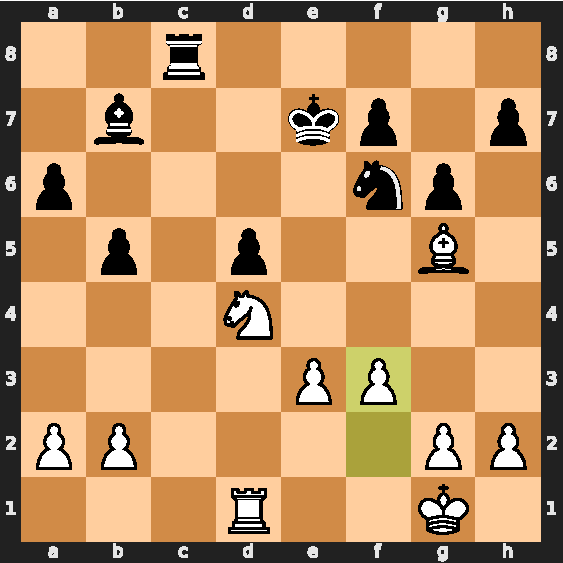
\includegraphics[width=\boardwidth]{diagrams/board-bcc641466549}}}

\Move{\href{https://lichess.org/analysis/pgn/d4_d5_Nf3_Nf6_c4_e6_Bg5_Be7_Nc3_Nbd7_e3_O-O_Rc1_b6_cxd5_exd5_Bb5_Bb7_O-O_a6_Ba4_Rc8_Qe2_c5_dxc5_Nxc5_Rfd1_Nxa4_Nxa4_b5_Rxc8_Qxc8_Nc3_Qc4_Nd4_Qxe2_Ncxe2_Rc8_Nf5_Kf8_Nxe7_Kxe7_Nd4_g6_f3_h6}{23...h6}}

Black could do nothing else except mark time with his Rook along the open file, since as soon as he moved away White would take it. White, on the other hand, threatens to march up with his King to e5 via f2, g3, f4, after having, of course, prepared the way. Hence, Black's best chance was to give up a Pawn, as in the text, in order to free his Knight.

\Move{\href{https://lichess.org/analysis/pgn/d4_d5_Nf3_Nf6_c4_e6_Bg5_Be7_Nc3_Nbd7_e3_O-O_Rc1_b6_cxd5_exd5_Bb5_Bb7_O-O_a6_Ba4_Rc8_Qe2_c5_dxc5_Nxc5_Rfd1_Nxa4_Nxa4_b5_Rxc8_Qxc8_Nc3_Qc4_Nd4_Qxe2_Ncxe2_Rc8_Nf5_Kf8_Nxe7_Kxe7_Nd4_g6_f3_h6_Bxh6}{24.\figB xh6} \href{https://lichess.org/analysis/pgn/d4_d5_Nf3_Nf6_c4_e6_Bg5_Be7_Nc3_Nbd7_e3_O-O_Rc1_b6_cxd5_exd5_Bb5_Bb7_O-O_a6_Ba4_Rc8_Qe2_c5_dxc5_Nxc5_Rfd1_Nxa4_Nxa4_b5_Rxc8_Qxc8_Nc3_Qc4_Nd4_Qxe2_Ncxe2_Rc8_Nf5_Kf8_Nxe7_Kxe7_Nd4_g6_f3_h6_Bxh6_Nd7}{\figN d7} \href{https://lichess.org/analysis/pgn/d4_d5_Nf3_Nf6_c4_e6_Bg5_Be7_Nc3_Nbd7_e3_O-O_Rc1_b6_cxd5_exd5_Bb5_Bb7_O-O_a6_Ba4_Rc8_Qe2_c5_dxc5_Nxc5_Rfd1_Nxa4_Nxa4_b5_Rxc8_Qxc8_Nc3_Qc4_Nd4_Qxe2_Ncxe2_Rc8_Nf5_Kf8_Nxe7_Kxe7_Nd4_g6_f3_h6_Bxh6_Nd7_h4}{25.h4} \href{https://lichess.org/analysis/pgn/d4_d5_Nf3_Nf6_c4_e6_Bg5_Be7_Nc3_Nbd7_e3_O-O_Rc1_b6_cxd5_exd5_Bb5_Bb7_O-O_a6_Ba4_Rc8_Qe2_c5_dxc5_Nxc5_Rfd1_Nxa4_Nxa4_b5_Rxc8_Qxc8_Nc3_Qc4_Nd4_Qxe2_Ncxe2_Rc8_Nf5_Kf8_Nxe7_Kxe7_Nd4_g6_f3_h6_Bxh6_Nd7_h4_Nc5}{\figN c5} \href{https://lichess.org/analysis/pgn/d4_d5_Nf3_Nf6_c4_e6_Bg5_Be7_Nc3_Nbd7_e3_O-O_Rc1_b6_cxd5_exd5_Bb5_Bb7_O-O_a6_Ba4_Rc8_Qe2_c5_dxc5_Nxc5_Rfd1_Nxa4_Nxa4_b5_Rxc8_Qxc8_Nc3_Qc4_Nd4_Qxe2_Ncxe2_Rc8_Nf5_Kf8_Nxe7_Kxe7_Nd4_g6_f3_h6_Bxh6_Nd7_h4_Nc5_Bf4}{26.\figB f4} \href{https://lichess.org/analysis/pgn/d4_d5_Nf3_Nf6_c4_e6_Bg5_Be7_Nc3_Nbd7_e3_O-O_Rc1_b6_cxd5_exd5_Bb5_Bb7_O-O_a6_Ba4_Rc8_Qe2_c5_dxc5_Nxc5_Rfd1_Nxa4_Nxa4_b5_Rxc8_Qxc8_Nc3_Qc4_Nd4_Qxe2_Ncxe2_Rc8_Nf5_Kf8_Nxe7_Kxe7_Nd4_g6_f3_h6_Bxh6_Nd7_h4_Nc5_Bf4_Ne6}{\figN e6}}

Black exchanges Knights to remain with Bishops of opposite colours, which gives him the best chance to draw.

\Move{\href{https://lichess.org/analysis/pgn/d4_d5_Nf3_Nf6_c4_e6_Bg5_Be7_Nc3_Nbd7_e3_O-O_Rc1_b6_cxd5_exd5_Bb5_Bb7_O-O_a6_Ba4_Rc8_Qe2_c5_dxc5_Nxc5_Rfd1_Nxa4_Nxa4_b5_Rxc8_Qxc8_Nc3_Qc4_Nd4_Qxe2_Ncxe2_Rc8_Nf5_Kf8_Nxe7_Kxe7_Nd4_g6_f3_h6_Bxh6_Nd7_h4_Nc5_Bf4_Ne6_Nxe6}{27.\figN xe6} \href{https://lichess.org/analysis/pgn/d4_d5_Nf3_Nf6_c4_e6_Bg5_Be7_Nc3_Nbd7_e3_O-O_Rc1_b6_cxd5_exd5_Bb5_Bb7_O-O_a6_Ba4_Rc8_Qe2_c5_dxc5_Nxc5_Rfd1_Nxa4_Nxa4_b5_Rxc8_Qxc8_Nc3_Qc4_Nd4_Qxe2_Ncxe2_Rc8_Nf5_Kf8_Nxe7_Kxe7_Nd4_g6_f3_h6_Bxh6_Nd7_h4_Nc5_Bf4_Ne6_Nxe6_Kxe6}{\figK xe6}}

\href{https://lichess.org/analysis/pgn/d4_d5_Nf3_Nf6_c4_e6_Bg5_Be7_Nc3_Nbd7_e3_O-O_Rc1_b6_cxd5_exd5_Bb5_Bb7_O-O_a6_Ba4_Rc8_Qe2_c5_dxc5_Nxc5_Rfd1_Nxa4_Nxa4_b5_Rxc8_Qxc8_Nc3_Qc4_Nd4_Qxe2_Ncxe2_Rc8_Nf5_Kf8_Nxe7_Kxe7_Nd4_g6_f3_h6_Bxh6_Nd7_h4_Nc5_Bf4_Ne6_Nxe6_fxe6}{27...fxe6} would be worse, as White would then be able to post his Bishop at e5.

\Move{\href{https://lichess.org/analysis/pgn/d4_d5_Nf3_Nf6_c4_e6_Bg5_Be7_Nc3_Nbd7_e3_O-O_Rc1_b6_cxd5_exd5_Bb5_Bb7_O-O_a6_Ba4_Rc8_Qe2_c5_dxc5_Nxc5_Rfd1_Nxa4_Nxa4_b5_Rxc8_Qxc8_Nc3_Qc4_Nd4_Qxe2_Ncxe2_Rc8_Nf5_Kf8_Nxe7_Kxe7_Nd4_g6_f3_h6_Bxh6_Nd7_h4_Nc5_Bf4_Ne6_Nxe6_Kxe6_Rd2}{28.\figR d2} \href{https://lichess.org/analysis/pgn/d4_d5_Nf3_Nf6_c4_e6_Bg5_Be7_Nc3_Nbd7_e3_O-O_Rc1_b6_cxd5_exd5_Bb5_Bb7_O-O_a6_Ba4_Rc8_Qe2_c5_dxc5_Nxc5_Rfd1_Nxa4_Nxa4_b5_Rxc8_Qxc8_Nc3_Qc4_Nd4_Qxe2_Ncxe2_Rc8_Nf5_Kf8_Nxe7_Kxe7_Nd4_g6_f3_h6_Bxh6_Nd7_h4_Nc5_Bf4_Ne6_Nxe6_Kxe6_Rd2_Rh8}{\figR h8}}

\ChessDiagram{\href{https://lichess.org/analysis/pgn/d4_d5_Nf3_Nf6_c4_e6_Bg5_Be7_Nc3_Nbd7_e3_O-O_Rc1_b6_cxd5_exd5_Bb5_Bb7_O-O_a6_Ba4_Rc8_Qe2_c5_dxc5_Nxc5_Rfd1_Nxa4_Nxa4_b5_Rxc8_Qxc8_Nc3_Qc4_Nd4_Qxe2_Ncxe2_Rc8_Nf5_Kf8_Nxe7_Kxe7_Nd4_g6_f3_h6_Bxh6_Nd7_h4_Nc5_Bf4_Ne6_Nxe6_Kxe6_Rd2_Rh8}{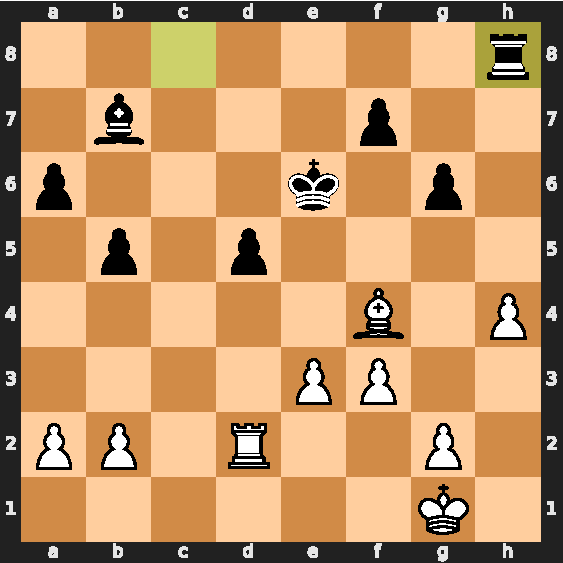
\includegraphics[width=\boardwidth]{diagrams/board-fb8d6b15f889}}}

Black wants to force \figB g3. g3 would be bad, on account of ...d4; which would get the Black Bishop into the game, even though White could answer e4. The text move is, however, weak, as will soon be seen. His best chance was to play ...b4; and follow it up with ...a5 and \figB a6. White meanwhile could play g4 and h5, obtaining a passed Pawn, which, with proper play, should win.

\Move{\href{https://lichess.org/analysis/pgn/d4_d5_Nf3_Nf6_c4_e6_Bg5_Be7_Nc3_Nbd7_e3_O-O_Rc1_b6_cxd5_exd5_Bb5_Bb7_O-O_a6_Ba4_Rc8_Qe2_c5_dxc5_Nxc5_Rfd1_Nxa4_Nxa4_b5_Rxc8_Qxc8_Nc3_Qc4_Nd4_Qxe2_Ncxe2_Rc8_Nf5_Kf8_Nxe7_Kxe7_Nd4_g6_f3_h6_Bxh6_Nd7_h4_Nc5_Bf4_Ne6_Nxe6_Kxe6_Rd2_Rh8_Rc2}{29.\figR c2!} \href{https://lichess.org/analysis/pgn/d4_d5_Nf3_Nf6_c4_e6_Bg5_Be7_Nc3_Nbd7_e3_O-O_Rc1_b6_cxd5_exd5_Bb5_Bb7_O-O_a6_Ba4_Rc8_Qe2_c5_dxc5_Nxc5_Rfd1_Nxa4_Nxa4_b5_Rxc8_Qxc8_Nc3_Qc4_Nd4_Qxe2_Ncxe2_Rc8_Nf5_Kf8_Nxe7_Kxe7_Nd4_g6_f3_h6_Bxh6_Nd7_h4_Nc5_Bf4_Ne6_Nxe6_Kxe6_Rd2_Rh8_Rc2_Rc8}{\figR c8} \href{https://lichess.org/analysis/pgn/d4_d5_Nf3_Nf6_c4_e6_Bg5_Be7_Nc3_Nbd7_e3_O-O_Rc1_b6_cxd5_exd5_Bb5_Bb7_O-O_a6_Ba4_Rc8_Qe2_c5_dxc5_Nxc5_Rfd1_Nxa4_Nxa4_b5_Rxc8_Qxc8_Nc3_Qc4_Nd4_Qxe2_Ncxe2_Rc8_Nf5_Kf8_Nxe7_Kxe7_Nd4_g6_f3_h6_Bxh6_Nd7_h4_Nc5_Bf4_Ne6_Nxe6_Kxe6_Rd2_Rh8_Rc2_Rc8_Rxc8}{30.\figR xc8} \href{https://lichess.org/analysis/pgn/d4_d5_Nf3_Nf6_c4_e6_Bg5_Be7_Nc3_Nbd7_e3_O-O_Rc1_b6_cxd5_exd5_Bb5_Bb7_O-O_a6_Ba4_Rc8_Qe2_c5_dxc5_Nxc5_Rfd1_Nxa4_Nxa4_b5_Rxc8_Qxc8_Nc3_Qc4_Nd4_Qxe2_Ncxe2_Rc8_Nf5_Kf8_Nxe7_Kxe7_Nd4_g6_f3_h6_Bxh6_Nd7_h4_Nc5_Bf4_Ne6_Nxe6_Kxe6_Rd2_Rh8_Rc2_Rc8_Rxc8_Bxc8}{\figB xc8}}

There are now Bishops of opposite colour, but nevertheless White has an easily-won game.

\Move{\href{https://lichess.org/analysis/pgn/d4_d5_Nf3_Nf6_c4_e6_Bg5_Be7_Nc3_Nbd7_e3_O-O_Rc1_b6_cxd5_exd5_Bb5_Bb7_O-O_a6_Ba4_Rc8_Qe2_c5_dxc5_Nxc5_Rfd1_Nxa4_Nxa4_b5_Rxc8_Qxc8_Nc3_Qc4_Nd4_Qxe2_Ncxe2_Rc8_Nf5_Kf8_Nxe7_Kxe7_Nd4_g6_f3_h6_Bxh6_Nd7_h4_Nc5_Bf4_Ne6_Nxe6_Kxe6_Rd2_Rh8_Rc2_Rc8_Rxc8_Bxc8_Kf2}{31.\figK f2}}

\ChessDiagram{\href{https://lichess.org/analysis/pgn/d4_d5_Nf3_Nf6_c4_e6_Bg5_Be7_Nc3_Nbd7_e3_O-O_Rc1_b6_cxd5_exd5_Bb5_Bb7_O-O_a6_Ba4_Rc8_Qe2_c5_dxc5_Nxc5_Rfd1_Nxa4_Nxa4_b5_Rxc8_Qxc8_Nc3_Qc4_Nd4_Qxe2_Ncxe2_Rc8_Nf5_Kf8_Nxe7_Kxe7_Nd4_g6_f3_h6_Bxh6_Nd7_h4_Nc5_Bf4_Ne6_Nxe6_Kxe6_Rd2_Rh8_Rc2_Rc8_Rxc8_Bxc8_Kf2}{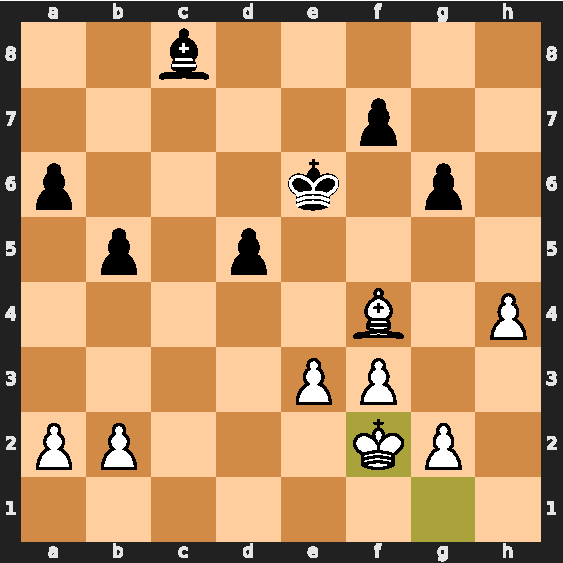
\includegraphics[width=\boardwidth]{diagrams/board-f52968d76963}}}

\Move{\href{https://lichess.org/analysis/pgn/d4_d5_Nf3_Nf6_c4_e6_Bg5_Be7_Nc3_Nbd7_e3_O-O_Rc1_b6_cxd5_exd5_Bb5_Bb7_O-O_a6_Ba4_Rc8_Qe2_c5_dxc5_Nxc5_Rfd1_Nxa4_Nxa4_b5_Rxc8_Qxc8_Nc3_Qc4_Nd4_Qxe2_Ncxe2_Rc8_Nf5_Kf8_Nxe7_Kxe7_Nd4_g6_f3_h6_Bxh6_Nd7_h4_Nc5_Bf4_Ne6_Nxe6_Kxe6_Rd2_Rh8_Rc2_Rc8_Rxc8_Bxc8_Kf2_d4}{31...d4}}

Practically forced. Otherwise the White King would march up to d4 and then to c5 and win Black's Queen's side Pawns. If Black attempted to stop this by putting his King at c6 then the White King would enter through e5 into Black's King's side and win just as easily.

\Move{\href{https://lichess.org/analysis/pgn/d4_d5_Nf3_Nf6_c4_e6_Bg5_Be7_Nc3_Nbd7_e3_O-O_Rc1_b6_cxd5_exd5_Bb5_Bb7_O-O_a6_Ba4_Rc8_Qe2_c5_dxc5_Nxc5_Rfd1_Nxa4_Nxa4_b5_Rxc8_Qxc8_Nc3_Qc4_Nd4_Qxe2_Ncxe2_Rc8_Nf5_Kf8_Nxe7_Kxe7_Nd4_g6_f3_h6_Bxh6_Nd7_h4_Nc5_Bf4_Ne6_Nxe6_Kxe6_Rd2_Rh8_Rc2_Rc8_Rxc8_Bxc8_Kf2_d4_exd4}{32.exd4} \href{https://lichess.org/analysis/pgn/d4_d5_Nf3_Nf6_c4_e6_Bg5_Be7_Nc3_Nbd7_e3_O-O_Rc1_b6_cxd5_exd5_Bb5_Bb7_O-O_a6_Ba4_Rc8_Qe2_c5_dxc5_Nxc5_Rfd1_Nxa4_Nxa4_b5_Rxc8_Qxc8_Nc3_Qc4_Nd4_Qxe2_Ncxe2_Rc8_Nf5_Kf8_Nxe7_Kxe7_Nd4_g6_f3_h6_Bxh6_Nd7_h4_Nc5_Bf4_Ne6_Nxe6_Kxe6_Rd2_Rh8_Rc2_Rc8_Rxc8_Bxc8_Kf2_d4_exd4_Kd5}{\figK d5} \href{https://lichess.org/analysis/pgn/d4_d5_Nf3_Nf6_c4_e6_Bg5_Be7_Nc3_Nbd7_e3_O-O_Rc1_b6_cxd5_exd5_Bb5_Bb7_O-O_a6_Ba4_Rc8_Qe2_c5_dxc5_Nxc5_Rfd1_Nxa4_Nxa4_b5_Rxc8_Qxc8_Nc3_Qc4_Nd4_Qxe2_Ncxe2_Rc8_Nf5_Kf8_Nxe7_Kxe7_Nd4_g6_f3_h6_Bxh6_Nd7_h4_Nc5_Bf4_Ne6_Nxe6_Kxe6_Rd2_Rh8_Rc2_Rc8_Rxc8_Bxc8_Kf2_d4_exd4_Kd5_Ke3}{33.\figK e3} \href{https://lichess.org/analysis/pgn/d4_d5_Nf3_Nf6_c4_e6_Bg5_Be7_Nc3_Nbd7_e3_O-O_Rc1_b6_cxd5_exd5_Bb5_Bb7_O-O_a6_Ba4_Rc8_Qe2_c5_dxc5_Nxc5_Rfd1_Nxa4_Nxa4_b5_Rxc8_Qxc8_Nc3_Qc4_Nd4_Qxe2_Ncxe2_Rc8_Nf5_Kf8_Nxe7_Kxe7_Nd4_g6_f3_h6_Bxh6_Nd7_h4_Nc5_Bf4_Ne6_Nxe6_Kxe6_Rd2_Rh8_Rc2_Rc8_Rxc8_Bxc8_Kf2_d4_exd4_Kd5_Ke3_Be6}{\figB e6} \href{https://lichess.org/analysis/pgn/d4_d5_Nf3_Nf6_c4_e6_Bg5_Be7_Nc3_Nbd7_e3_O-O_Rc1_b6_cxd5_exd5_Bb5_Bb7_O-O_a6_Ba4_Rc8_Qe2_c5_dxc5_Nxc5_Rfd1_Nxa4_Nxa4_b5_Rxc8_Qxc8_Nc3_Qc4_Nd4_Qxe2_Ncxe2_Rc8_Nf5_Kf8_Nxe7_Kxe7_Nd4_g6_f3_h6_Bxh6_Nd7_h4_Nc5_Bf4_Ne6_Nxe6_Kxe6_Rd2_Rh8_Rc2_Rc8_Rxc8_Bxc8_Kf2_d4_exd4_Kd5_Ke3_Be6_Kd3}{34.\figK d3} \href{https://lichess.org/analysis/pgn/d4_d5_Nf3_Nf6_c4_e6_Bg5_Be7_Nc3_Nbd7_e3_O-O_Rc1_b6_cxd5_exd5_Bb5_Bb7_O-O_a6_Ba4_Rc8_Qe2_c5_dxc5_Nxc5_Rfd1_Nxa4_Nxa4_b5_Rxc8_Qxc8_Nc3_Qc4_Nd4_Qxe2_Ncxe2_Rc8_Nf5_Kf8_Nxe7_Kxe7_Nd4_g6_f3_h6_Bxh6_Nd7_h4_Nc5_Bf4_Ne6_Nxe6_Kxe6_Rd2_Rh8_Rc2_Rc8_Rxc8_Bxc8_Kf2_d4_exd4_Kd5_Ke3_Be6_Kd3_Kc6}{\figK c6} \href{https://lichess.org/analysis/pgn/d4_d5_Nf3_Nf6_c4_e6_Bg5_Be7_Nc3_Nbd7_e3_O-O_Rc1_b6_cxd5_exd5_Bb5_Bb7_O-O_a6_Ba4_Rc8_Qe2_c5_dxc5_Nxc5_Rfd1_Nxa4_Nxa4_b5_Rxc8_Qxc8_Nc3_Qc4_Nd4_Qxe2_Ncxe2_Rc8_Nf5_Kf8_Nxe7_Kxe7_Nd4_g6_f3_h6_Bxh6_Nd7_h4_Nc5_Bf4_Ne6_Nxe6_Kxe6_Rd2_Rh8_Rc2_Rc8_Rxc8_Bxc8_Kf2_d4_exd4_Kd5_Ke3_Be6_Kd3_Kc6_a3}{35.a3} \href{https://lichess.org/analysis/pgn/d4_d5_Nf3_Nf6_c4_e6_Bg5_Be7_Nc3_Nbd7_e3_O-O_Rc1_b6_cxd5_exd5_Bb5_Bb7_O-O_a6_Ba4_Rc8_Qe2_c5_dxc5_Nxc5_Rfd1_Nxa4_Nxa4_b5_Rxc8_Qxc8_Nc3_Qc4_Nd4_Qxe2_Ncxe2_Rc8_Nf5_Kf8_Nxe7_Kxe7_Nd4_g6_f3_h6_Bxh6_Nd7_h4_Nc5_Bf4_Ne6_Nxe6_Kxe6_Rd2_Rh8_Rc2_Rc8_Rxc8_Bxc8_Kf2_d4_exd4_Kd5_Ke3_Be6_Kd3_Kc6_a3_Bc4}{\figB c4+} \href{https://lichess.org/analysis/pgn/d4_d5_Nf3_Nf6_c4_e6_Bg5_Be7_Nc3_Nbd7_e3_O-O_Rc1_b6_cxd5_exd5_Bb5_Bb7_O-O_a6_Ba4_Rc8_Qe2_c5_dxc5_Nxc5_Rfd1_Nxa4_Nxa4_b5_Rxc8_Qxc8_Nc3_Qc4_Nd4_Qxe2_Ncxe2_Rc8_Nf5_Kf8_Nxe7_Kxe7_Nd4_g6_f3_h6_Bxh6_Nd7_h4_Nc5_Bf4_Ne6_Nxe6_Kxe6_Rd2_Rh8_Rc2_Rc8_Rxc8_Bxc8_Kf2_d4_exd4_Kd5_Ke3_Be6_Kd3_Kc6_a3_Bc4_Ke3}{36.\figK e3} \href{https://lichess.org/analysis/pgn/d4_d5_Nf3_Nf6_c4_e6_Bg5_Be7_Nc3_Nbd7_e3_O-O_Rc1_b6_cxd5_exd5_Bb5_Bb7_O-O_a6_Ba4_Rc8_Qe2_c5_dxc5_Nxc5_Rfd1_Nxa4_Nxa4_b5_Rxc8_Qxc8_Nc3_Qc4_Nd4_Qxe2_Ncxe2_Rc8_Nf5_Kf8_Nxe7_Kxe7_Nd4_g6_f3_h6_Bxh6_Nd7_h4_Nc5_Bf4_Ne6_Nxe6_Kxe6_Rd2_Rh8_Rc2_Rc8_Rxc8_Bxc8_Kf2_d4_exd4_Kd5_Ke3_Be6_Kd3_Kc6_a3_Bc4_Ke3_Be6}{\figB e6} \href{https://lichess.org/analysis/pgn/d4_d5_Nf3_Nf6_c4_e6_Bg5_Be7_Nc3_Nbd7_e3_O-O_Rc1_b6_cxd5_exd5_Bb5_Bb7_O-O_a6_Ba4_Rc8_Qe2_c5_dxc5_Nxc5_Rfd1_Nxa4_Nxa4_b5_Rxc8_Qxc8_Nc3_Qc4_Nd4_Qxe2_Ncxe2_Rc8_Nf5_Kf8_Nxe7_Kxe7_Nd4_g6_f3_h6_Bxh6_Nd7_h4_Nc5_Bf4_Ne6_Nxe6_Kxe6_Rd2_Rh8_Rc2_Rc8_Rxc8_Bxc8_Kf2_d4_exd4_Kd5_Ke3_Be6_Kd3_Kc6_a3_Bc4_Ke3_Be6_Bh6}{37.\figB h6}}

It is better not to hurry \href{https://lichess.org/analysis/pgn/d4_d5_Nf3_Nf6_c4_e6_Bg5_Be7_Nc3_Nbd7_e3_O-O_Rc1_b6_cxd5_exd5_Bb5_Bb7_O-O_a6_Ba4_Rc8_Qe2_c5_dxc5_Nxc5_Rfd1_Nxa4_Nxa4_b5_Rxc8_Qxc8_Nc3_Qc4_Nd4_Qxe2_Ncxe2_Rc8_Nf5_Kf8_Nxe7_Kxe7_Nd4_g6_f3_h6_Bxh6_Nd7_h4_Nc5_Bf4_Ne6_Nxe6_Kxe6_Rd2_Rh8_Rc2_Rc8_Rxc8_Bxc8_Kf2_d4_exd4_Kd5_Ke3_Be6_Kd3_Kc6_a3_Bc4_Ke3_Be6_g4}{37.g4} because of ...f5; for although White could win in any case, it would take longer. Now the White King threatens to help by going in through f4 after posting the Bishop at g7, where it not only protects the d-pawn, but indirectly also the b-pawn.

\Move{\href{https://lichess.org/analysis/pgn/d4_d5_Nf3_Nf6_c4_e6_Bg5_Be7_Nc3_Nbd7_e3_O-O_Rc1_b6_cxd5_exd5_Bb5_Bb7_O-O_a6_Ba4_Rc8_Qe2_c5_dxc5_Nxc5_Rfd1_Nxa4_Nxa4_b5_Rxc8_Qxc8_Nc3_Qc4_Nd4_Qxe2_Ncxe2_Rc8_Nf5_Kf8_Nxe7_Kxe7_Nd4_g6_f3_h6_Bxh6_Nd7_h4_Nc5_Bf4_Ne6_Nxe6_Kxe6_Rd2_Rh8_Rc2_Rc8_Rxc8_Bxc8_Kf2_d4_exd4_Kd5_Ke3_Be6_Kd3_Kc6_a3_Bc4_Ke3_Be6_Bh6_Kd5}{37...\figK d5} \href{https://lichess.org/analysis/pgn/d4_d5_Nf3_Nf6_c4_e6_Bg5_Be7_Nc3_Nbd7_e3_O-O_Rc1_b6_cxd5_exd5_Bb5_Bb7_O-O_a6_Ba4_Rc8_Qe2_c5_dxc5_Nxc5_Rfd1_Nxa4_Nxa4_b5_Rxc8_Qxc8_Nc3_Qc4_Nd4_Qxe2_Ncxe2_Rc8_Nf5_Kf8_Nxe7_Kxe7_Nd4_g6_f3_h6_Bxh6_Nd7_h4_Nc5_Bf4_Ne6_Nxe6_Kxe6_Rd2_Rh8_Rc2_Rc8_Rxc8_Bxc8_Kf2_d4_exd4_Kd5_Ke3_Be6_Kd3_Kc6_a3_Bc4_Ke3_Be6_Bh6_Kd5_Bg7}{38.\figB g7}}

\noindent\textbf{Resigns.}

The student ought to have realised by this time the enormous importance of playing well every kind of ending. In this game again, practically from the opening, White aimed at nothing but the isolation of Black's d-pawn. Once he obtained that, he tried for and obtained, fortunately, another advantage of position elsewhere which translated itself into the material advantage of a Pawn. Then by accurate playing in the ending he gradually forced home his advantage. This ending has the merit of having been played against one of the finest players in the world.

\end{document}
